\documentclass[reprint,aps,prl,amsmath,amssymb,superscriptaddress,showpacs]{revtex4-1}
\usepackage{tikz,graphicx,url,float}
\usetikzlibrary{arrows}

\usepackage{amsthm}
\newtheorem{definition}{Definition}
\newtheorem{theorem}{Theorem}

\begin{document}

\title{An approximation to the end date distribution of project networks}

\author{Alexei Vazquez}
\email{alexei@nodeslinks.com}
\affiliation{Nodes \& Links}


\date{\today}

\begin{abstract}
A project is represented by a directed acyclic graph. Nodes represent activities and arcs indicate precedence relations. A project end date is stablished during planning using as input the project network and the activity durations. However, adverse events increase activity durations, causing delay cascades and shifting the project end date. Here I derive an approximate analytical formula for the end date distribution. This approximation works when both the activity durations and delays follow sub-exponential distributions.   
\end{abstract}

\maketitle

%\begin{figure}[t]
%\includegraphics[width=5in]{auxo_fig_model.eps}
%\caption{}
%\label{fig_model}
%\end{figure}

%\section{Introduction}

Let $P(V,E,\vec{d})$ be a project with a set of activities $V$, a set of activity relations $E$ and a vector of activity durations $\vec{d}$. The project start and end are represented by the activities $i=0$ and $i=n$, respectively, of duration zero. An arc $i\rightarrow j\in E$ indicates that $i$ must finish before $j$ starts, what is called a finish-start relation. Project networks have other relation types \cite{van13}. For simplicity I will limit the analysis to finish-start relations. I will denote by $I_i=\{j|j\rightarrow i\rin E$ the set of predecesors a. Logical consistence implies that the project network is a directed acyclic graph.  The nodes in a directed acyclic graph can be ordered topologically such that if $i\rightarrow j$ then $i$ is before $j$ in the topological order, for all $i\rightarrow j\in E$.

The earliest an activity can finish is determined by the recursive relation
%
\begin{equation}
x_i = \max_{j\in I_i} x_j + d_i\ ,
\label{forward} 
\end{equation}
%
with the boundary condition $x_0=s$, where $s$ is the start date. We calculate $\vec{x}$ Performing a forward pass of  Eq. (\ref{forward}) along the topological order. Next we do backward propagation to calculate the latest an activity can finish without altering the project en date
%
\begin{equation}
y_i = \min_{j \in O_i} \left(y_j - d_i\right)\ ,
\label{backward} 
\end{equation}
%
with the boundary condition $y_n=x_n$. $\vec{x}$ and $\vec{y}$ set the early and late start dates for every activity. If $i\in I_j$ then the difference 
%
\begin{equation}
w_{ij} = x_i - y_j\ ,
\label{w}
\end{equation}
%
is the free float between the two activities \cite{van13}. The maximum delay at activity $i$ without shifting the finish date of activity $j$. In turn we can determine the amount of delay tolerated at a given activity without causing a shift in the project end date. This is called to total float and is calculated as follows
%
\begin{equation}
T_{n,i} = x_i-y_i\ .
\label{Tn} 
\end{equation}
%
The subscript $n$ emphasises that $T_{in}$ is the total float from activity $i$ to the project end. This will be later generalised to any pair of activities. The process of planning for the shortest time generates one or more critical paths. Paths of activities with $T_{in}=0$ from the start to the end activity. Finally, note that I have adopted a negative sign for the free floats and the total floats. I do so to emphasise the intuition that floats subtract delay. Yet, bear in mind that in the main stream literature they are defined as positive \cite{van13}.

In practice exogenous factors delay the start of activities of increase their durations. If the delay on finishing an activity exceeds one or more of the free floats with predecessor activities, it will cause their delay as well, starting a delay cascade. The delay cascade can reach the project end activity causing a delay of the project end date. Risk models are developed to determine the distribution of project end dates given models of delay for each activity. These models are then investigated by means of numerical simulations and summary statistics are reported. Here I follow an analytical approach.

Let $\vec{h}$ represent the vector of activity delays caused by exogenous factors and $\vec{z}$ the vactor of activity delays after the propagation of the exogenous delays. The delays propagate via a recursive equation similar to Eq. (\ref{forward}), with some twists
 %
\begin{equation}
z_i = f\left\{\max_{j\in I_i} \left[\max(0,z_j+w_{ji})\right] , h_i\right\}\ .
\label{forward_delay} 
\end{equation}
% 
The term $\max(0,z_j-w_{ji})$ accounts for the fact that delays are passed on only if they exceed the free float between the activities. Then we take the maximum delay passed from all the incoming relations to activity $i$. Finally, the function $f_i(x,y)$ takes care of merging the delays coming from predecessors and from exogenous sources. If all exogenous delays act on the activity start, then they can be modelled as a finish-start relation, obtaining $f_i(x,y)=\max(x,y)$. If all exogenous delays act on the activity duration, then they can be modelled as added delays $f_i(x,y)=x+y$. Even a unique contingency such as an adverse weather event can act differently depending on where does it falls in the calendar relative to some activity. If it falls before the activity start, it competes with delays from predecessors a s a cause of delay for the activity start. If the adverse weather event happens while the activity is in execution it will delay its finish date on top of any delay coming from predecessor activities. In general, the best we can say is the inequalities
%
\begin{equation}
\max(x,y)\leq f_i(x,y)\leq x+y\ .
\label{f_bounds}
\end{equation}
%
This modelling challenge would require an agent based approach with detailed specifications of $f_i(x,y)$ at every activity. Yet, when $x$ and $y$ follow sub-exponential distributions $\max(x,y)\approx x+y$. If that is the case then $f_i(x,y)\approx \max(x,y)\approx x+y$ and the problem is solved. 

Sub-exponential distributions cannot be bounded by any exponential function $f(x) = e^{-\alpha x}$  when $x\rightarrow\infty$ \cite{foss13}. If we take two random variables $x$ and $y$ generated from the same sub-exponential distribution then ${\rm Pr}(x+y>z)\sim {\rm Pr}\max(x,y)>z$ when $z\rightarrow\infty$. The only way that $x+y$ is larger than $z$ is that either $x$ or $y$ are larger than $z$. We cannot take this result as grated when we propagate delays in the activity network. The errors could accumulate when the delay propagation takes several steps and we also need to take into account the free floats that act as delay sinks. In the following I explore different scenarios by means of numerical simulations. I investigate the difference in using $\max(x,y$ and $x+y$ by means of numerical simulations.

We need a model to generate project networks, a model to generate activity durations and a model to generate exogenous delays. For the exogenous delay we will assume a member of the sub-exponential distribution class, the log-normal distribution $p(h)\sim e^{-[log(h/\mu)]^2/2\sigma^2}/h$. For the activity durations we will explore different choices. We will generate project networks using the duplication-split model \cite{vazquez22}. In this model, we start with two activities representing the project start and end, with an arc from start to end. Then, at each discrete step, we select an activity with uniform probability across all current activities (the parent) and create a new activity (the daughter). With probability $q$ the daughter is a duplicate of the parent, inheriting all the incoming and outgoing relations from the parent activity. Otherwise, the parent transfer all the outgoing arcs to the daughter and creates an arc from the parent to the daughter. We call $q$ the duplicate rate.  It is demonstrated that both the in-degree and out-degree distribution has a power law tail with exponent $1/q$ and the network diameter grows at least as $n^{1-q}$ \cite{vazquez22}. As we tune $q$ from 0 to 1 we change from networks that are quasi-linear and have narrow degree distributions to networks with wide degree distributions and multiple parallel paths.

The simulations proceed as follow. The inputs are the number of activities $n$, the duplication rate $q$, the distributions of activity durations $p(d)$ and the exogenous delay distribution $p(h)$. We reiterate teh focus on sub-exponentially distributed exogenous delays, so I choose the log-normal $p(h)\sim e^{-[log(h/\mu)]^2/2\sigma^2}/h$ with $\mu=1$. First, we generate a duplication-split network  with parameters $(n,q)$. Second, we assign durations to activity from $p(d)$. and run Eqs. (\ref{forward})-(\ref{w}) to generate the free floats $w$. Third, we generate random delays from $p(h)$ and run Eq. (\ref{forward_delay}) with apre-defined $f(x,y)$ to calculate $z_n$, the project end delay. We repeat this third step to generate $z_n$ samples. From that list of samples we report the value of $z_n$ above 80\% of all samples. This quantity is commonly used in project management and it is named the project $p80$. Fourth, for each parameter set $\{n,q,p(d),f(x,y)\}_i$ we generate multiple $p80$ values $\pi(f)_i$ by sampling over realisations of the network and activity durations. We do that for $f(x,y)=\max(x,y)$ and $f(x,y)=x+y$. Finally, we calculate the slope through the origin
%
\begin{equation}
S = \frac{ \sum_i \pi(f_{\max})_i \pi(f_{\rm sum})_i }{ \sum_i [\pi(f_{\max})_i]^2 }
\label{slope}
\end{equation}
%
Since $x+y\geq\max(x,y)$ then $S\geq1$. The question is how close to 1.

\begin{figure}[t]
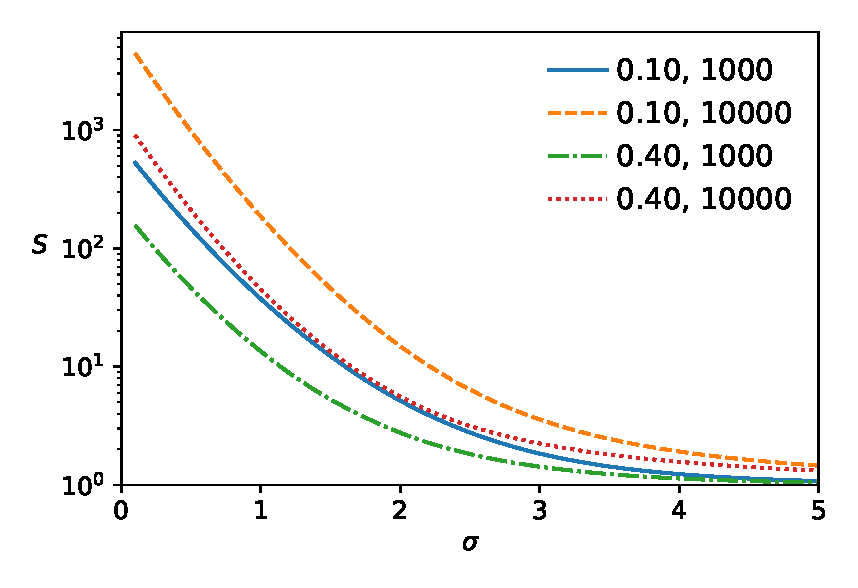
\includegraphics[width=3.3in]{maxsum.scheduling.dupsplit.arc_distribution_zero.eps}
\caption{}
\label{fig1}
\end{figure}

If we set activity durations to zero (or to any constant) we can investigate how the differences between $\max(x,y)$ and $x+y$ propagate without the additional complication of the free float weights $w$. Given the log-normal $p(h)\sim e^{-[log(h/\mu)]^2/2\sigma^2}/h$, we expect $S\rightarrow1$ when $\sigma\rightarrow\infty$. This asymptotic behaviour is corroborated in Fig. \ref{fig1}. However, the convergence is very slow. We need $\sigma>3$ to attain $S<2$. Bear in mind that the variance of the log-normal distribution is order $e^{\sigma^2}$. For example, $\sigma=3$ implies a variance of order $e^9\approx 8000$. We can conclude that, if the activity durations are homogeneous, then $f(x,y)=\max(x,y)$ is a poor lower bound for $f(x,y)=x+y$. I similar picture is obtained using $p(d)\sim e^{-d/\mu^\prime}$. The same is expected for any exponentially bound distribution.

\begin{figure}[t]
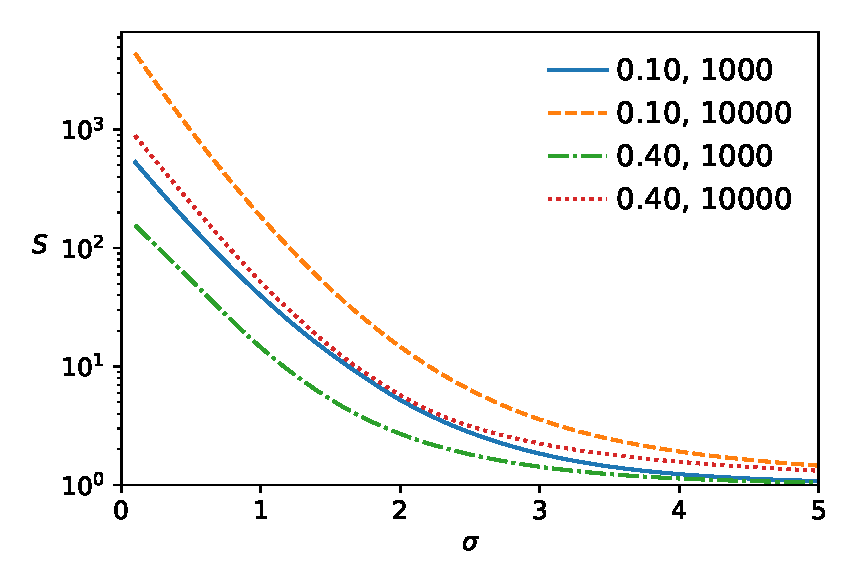
\includegraphics[width=3.3in]{maxsum.scheduling.dupsplit.arc_distribution_lognormal.arc_sigma_1.eps}
\caption{}
\label{fig2}
\end{figure}

The picture changes if the activity durations follow a sub-exponential distribution as well. For example, a log-normal distribution $p(d)\sim e^{-[log(d/\mu^\prime)]^2/2\sigma^{\prime 2}}/d$. I will set $\mu^\prime=1$ since $\sigma^\prime$ controls the shape of the distribution tail. For $\sigma^\prime=1$ we obtain the plot in Fig. \ref{fig2}. For $\sigma<1$ the value of $S$ is close or below 2. In this context $f_{\max}$ is a good approximation for $f_{\rm sum}$. As $\sigma$ approaches 1 the value of $S$ reaches a maximum and the decays towards $S=1$. The transition from $S\approx 1$ to $S\gg1$ around $\sigma=1$ becomes sharper with increasing the number of activities. 




If $f(x,y)=\max(x,y)$ gives similar results to $f(x)=x+y$ then we can choose either. As shown below, using  $f(x,y)=\max(x,y)$ has some advantages. Let us explore the case $f(x,y)=\max(x,y)$. We can solve Eq. (\ref{forward_delay}) iteratively
%
\begin{equation}
z_{i,t+1} = \max\left[ \max_{j\in I_i} \max(z_{j,t} + w_{ij}), h_i\right]\ ,
\label{forward_delay_iter} 
\end{equation}
%
with the initial condition $z_{i,0}=h_i$. Defining $w_{ii}=0$ we can rewrite the Eq. above to the more compact form
%
\begin{equation}
z_{i,t+1} = \max_{j\in I_i\cup\{i\}} ( z_{j,t} + w_{ij})\ .
\label{maxapp}
\end{equation}
%
The shape of this equation calls for the max-plus algebra \cite{butkovic10}. The max-plus algebra is defined by the semiring $(\mathbf{R}\cup\{-\infty\},\oplus,\otimes)$ with the sum operation defined as
$x\oplus y = \max(x,y)$ and the product as $x\otimes y = x+y$. The max-plus algebra has been used to investigate networks with cycles \cite{hei14}. For example, of transportation networks, where it is desired to have a route back and forward between any two nodes. Here the focus is on directed acyclic graphs. Using the max-plus algebra we rewrite  (\ref{maxapp}) as
%
\begin{equation}
\vec{z}_{t+1} = L\otimes \vec{z}_t\ ,
\label{maxplus} 
\end{equation}
%
where
%
\begin{equation}
L = \left\{
\begin{array}{ll}
0 & {\rm if}\ i=j\\
w_{ij} & {\rm if}\ j\in I_i\\
-\infty & {\rm otherwise}
\end{array}\right.
\label{L}
\end{equation}
%
is the local weights matrix. From now on we focus on the properties of $\vec{z}_t$ after several iterations of (\ref{maxplus}). The answer depends on what type of graph encodes the input sets 

Project networks are represented by directed acyclic graphs. Therefore, there is no path larger than the graph diameter $D$. After $D$ iterations starting from $\vec{z}_0=\vec{h}$ the system will reach the steady state solution
%
\begin{equation}
\vec{z}_{\infty} = T\otimes \vec{h}\ ,
\label{maxplus_oo} 
\end{equation}
%
where
%
\begin{equation}
T = W^{\otimes D}\ ,
\label{T}
\end{equation}
%
is the total float matrix. The element $-T_{ij}$ equals the maximum $h_i$ that yields $z_{j,\infty}=0$.

{\em Main result.} Calculating the cumulative distribution function for the delay at each activity is now straightforward. If $F_i(x)={\rm Pr}(h_i\leq x)$ and $G_i(x) = {\rm Pr}(z_{i,\infty}\leq x)$, then from Eq. (\ref{maxplus_oo}) we obtain
%
\begin{equation}
G_i(x) = \prod_{j} F_j(x+T_{ij})\ .
\label{CDF}
\end{equation}
%

The non-trivial region where $\max(x,y)$ is a good approximation to $x+y$ remains to be explained. Intuitively, if both the delays and the free floats have sub-exponential distributions, and we extract a delay and a free float from those distributions, then one of them will be much larger than the other with high probability. In that case, the delays that exceed the free floats will be large and $\max(x,y)$ is a good approximation for $x+y$.








\begin{figure}[t]
%\includegraphics[width=3.3in]{maxsum.scheduling.dupsplit.arc_distribution_lognormal.arc_sigma_5.eps}
\caption{}
\label{fig}
\end{figure}

%\section*{Conclusions}



\bibliographystyle{apsrev4-1}

\bibliography{maxplus.bib}

\end{document}
